
%(BEGIN_QUESTION)
% Copyright 2009, Tony R. Kuphaldt, released under the Creative Commons Attribution License (v 1.0)
% This means you may do almost anything with this work of mine, so long as you give me proper credit

Read and outline the ``Derivative Control Action'' subsection of the ``Pneumatic PID Controllers'' section of the ``Closed-Loop Control'' chapter in your {\it Lessons In Industrial Instrumentation} textbook.  Note the page numbers where important illustrations, photographs, equations, tables, and other relevant details are found.  Prepare to thoughtfully discuss with your instructor and classmates the concepts and examples explored in this reading.

\underbar{file i04313}
%(END_QUESTION)





%(BEGIN_ANSWER)


%(END_ANSWER)





%(BEGIN_NOTES)

Converting a proportional-only pneumatic controller to have derivative action is easy: simply place an adjustable restriction (valve) between the nozzle backpressure line and the feedback bellows.  This has the effect of delaying the balancing action of the feedback bellows, which causes the output to ``over-react'' to changes in input (error).  Specifically, the output pressure must assume a higher or lower value than it ordinarily would with proportional action alone, in order to keep air flowing through the restrictor valve and change the feedback bellows pressure.








\vskip 20pt \vbox{\hrule \hbox{\strut \vrule{} {\bf Suggestions for Socratic discussion} \vrule} \hrule}

\begin{itemize}
\item{} Set up and run a ``thought experiment'' to demonstrate how the mechanism implements derivate (rate) control action, in addition to proportional control action.
\item{} What would be the effect of fully opening the derivative valve in this mechanism?
\item{} What would be the effect of closing off the derivative valve in this mechanism?
\item{} What would be the effect of adding extra volume (capacity) to the output bellows in this mechanism?
\end{itemize}














\vfil \eject

\noindent
{\bf Prep Quiz:}

The adjustment designed to control the aggressiveness of {\it derivative} action (without affecting {\it integral} action) in this pneumatic controller is:

$$\includegraphics[width=15.5cm]{i04313x01.eps}$$

\begin{itemize}
\item{} Fulcrum position
\vskip 10pt
\item{} Regulator $PCV_1$
\vskip 10pt
\item{} Regulator $PCV_2$ 
\vskip 10pt
\item{} Valve $V_2$
\vskip 10pt
\item{} Auto/Manual selector
\vskip 10pt
\item{} Valve $V_1$
\end{itemize}



\vfil \eject

\noindent
{\bf Prep Quiz:}

The adjustment designed to control the aggressiveness of {\it integral} action (without affecting {\it derivative} action) in this pneumatic controller is:

$$\includegraphics[width=15.5cm]{i04313x01.eps}$$

\begin{itemize}
\item{} Fulcrum position
\vskip 10pt
\item{} Regulator $PCV_1$
\vskip 10pt
\item{} Regulator $PCV_2$ 
\vskip 10pt
\item{} Valve $V_2$
\vskip 10pt
\item{} Auto/Manual selector
\vskip 10pt
\item{} Valve $V_1$
\end{itemize}


%INDEX% Reading assignment: Lessons In Industrial Instrumentation, closed-loop control (Pneumatic controller derivative action)

%(END_NOTES)


